\chapter{The Dirac Sea, Fermion Mass, and Four-Component Spinors}

\section{Right-Moving Fermions and the Dirac Sea}

The Dirac equation is an equation for fermions. Relativistic bosons satisfy different equations, such as the Klein--Gordon equation or Maxwell's equations. The simplest example lives in one spatial dimension and initially describes particles and antiparticles that can move only to the right.

Begin with a plane wave,
\begin{equation}
\psi(x,t)=\psi_0 e^{i(kx-\omega t)}.
\end{equation}
Its phase velocity is
\begin{equation}
v_{\mathrm{ph}}=\frac{\omega}{k}.
\end{equation}
The signs of \(k\) and \(\omega\) matter. If they have the same sign, the phase moves to the right; if they have opposite signs, it moves to the left. When \(\omega\) is proportional to \(k\), the phase and group velocities coincide:
\begin{equation}
v_{\mathrm{g}}=\frac{d\omega}{dk}=\frac{\omega}{k}.
\end{equation}

Consider the first-order equation
\begin{equation}
\frac{\partial\psi}{\partial x}
+
\frac{\partial\psi}{\partial t}
=0.
\end{equation}
Substitution of the plane wave gives
\begin{equation}
ik\psi-i\omega\psi=0,
\end{equation}
and hence
\begin{equation}
\omega=k.
\end{equation}
The wave therefore moves to the right. It is useful to label the field accordingly:
\begin{equation}
\frac{\partial\psi_R}{\partial t}
=
-\frac{\partial\psi_R}{\partial x}.
\end{equation}

Restoring the speed of light gives the dimensional form
\begin{equation}
\frac{\partial\psi_R}{\partial x}
+
\frac{1}{c}\frac{\partial\psi_R}{\partial t}
=0,
\end{equation}
so that
\begin{equation}
\omega=ck.
\end{equation}
From now on \(c=1\). With \(\hbar=1\), \(\omega\) is also the energy of one quantum.

\begin{figure}[htbp]
\centering
\begin{tikzpicture}[scale=1.0]
\draw[->] (-3.1,0) -- (3.1,0) node[right] {$k$};
\draw[->] (0,-2.7) -- (0,2.7) node[above] {$\omega$};
\draw[thick] (-2.5,-2.5) -- (2.5,2.5);
\node[above left] at (2.35,2.35) {$\omega=k$};
\node[below right] at (2.45,0) {positive momentum};
\node[above left] at (-2.45,0) {negative momentum};
\node[right] at (0,2.25) {positive energy};
\node[left] at (0,-2.25) {negative energy};
\end{tikzpicture}
\caption{The massless right-moving dispersion \(\omega=k\) contains positive- and negative-energy branches.}
\end{figure}

The straight line has a serious consequence. Positive \(k\) gives positive energy, while negative \(k\) gives negative energy. Both parts nevertheless describe right-moving waves because \(\omega/k=1\) on the whole line.

An electron placed on the positive-energy part could fall to a lower state, emit a positive-energy photon, fall again, and continue down the spectrum: down one stair, then another, and another. No electron would be stable. More seriously, the world would lower its energy by producing more and more negative-energy electrons.

Fermionic exclusion supplies the cure. Fill every negative-energy electron state. No second electron can enter an already occupied state, so the completely filled negative-energy sector blocks an unlimited fall. This filled sector is the Dirac sea, and its completely filled state is the ground state, or vacuum.

\begin{classroomqa}
\lecturetimestamp{00:07:19}
\audiencequestion{Are there infinitely many lower negative-energy states?}
\lecturerresponse{Yes. With discrete momenta the spectrum is like an infinite staircase; with continuous momenta it is like a continuous slide. Filling the negative-energy sea prevents an electron from descending indefinitely, although a finite downward transition with photon emission may still be possible when an unoccupied lower state is available.}
\end{classroomqa}

This explains why an equation with this spectrum must be quantized as a fermionic theory. If the quanta were bosons, arbitrarily many of them could occupy the same lower state, and filling the negative-energy sector would not stabilize the vacuum.

The filled-sea picture also produces antiparticles. In the vacuum all negative-energy levels are occupied and all positive-energy levels are empty. An electron may be promoted from any occupied negative-energy level to any unoccupied positive-energy level; the initial and final levels need not be placed symmetrically.

\begin{figure}[htbp]
\centering
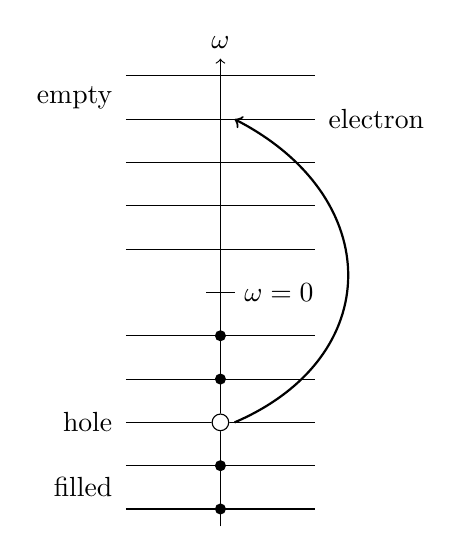
\begin{tikzpicture}[x=1cm,y=0.55cm]
\draw[->] (0,-5.4) -- (0,5.4) node[above] {$\omega$};
\draw (-0.18,0) -- (0.18,0) node[right] {$\omega=0$};
\foreach \y in {-5,-4,-3,-2,-1} {
  \draw (-1.2,\y) -- (1.2,\y);
  \fill (0,\y) circle (2pt);
}
\foreach \y in {1,2,3,4,5} {
  \draw (-1.2,\y) -- (1.2,\y);
}
\draw[->,thick] (0.18,-3) .. controls (2.1,-1.5) and (2.1,2.2) .. (0.18,4);
\draw[white,fill=white] (0,-3) circle (3pt);
\draw (0,-3) circle (3pt);
\node[left] at (-1.25,-3) {hole};
\node[left] at (-1.25,-4.5) {filled};
\node[left] at (-1.25,4.5) {empty};
\node[right] at (1.25,4) {electron};
\end{tikzpicture}
\caption{Promoting an occupied negative-energy electron produces a positive-energy electron and leaves a hole in the filled sea.}
\end{figure}

Removing an electron of negative energy raises the energy relative to the vacuum, so the hole has positive energy. On the branch \(\omega=k\), the removed electron also had negative momentum. Removing negative momentum leaves a positive excess of momentum, so the hole has positive momentum. With the electron charge taken to be negative, the missing electron has positive charge. Thus the hole is a positive-energy, positive-momentum antiparticle, while the promoted electron has negative charge, positive energy, and positive momentum. Every real excitation in this one-branch theory moves to the right.

The field \(\psi_R\) is built from fermionic creation and annihilation operators. The particle and hole interpretation is therefore a statement about the quanta created and removed by the field, not only about a classical wave.

There is still an asymmetry. The right-moving sea contains negative-energy states with negative momentum. Its formal total momentum is enormous and points to the left. One may define the vacuum momentum to be zero by subtracting that constant, but the state remains structurally unbalanced: particles and antiparticles move only to the right, while the filled vacuum is made from negative-momentum states.

\section{The Left-Moving Branch and a Balanced Vacuum}

Left-right balance requires a second, independent field with its own creation and annihilation operators. Let it satisfy
\begin{equation}
\frac{\partial\psi_L}{\partial t}
=
+\frac{\partial\psi_L}{\partial x}.
\end{equation}
For the same plane-wave form,
\begin{equation}
-i\omega\psi_L=ik\psi_L,
\end{equation}
so
\begin{equation}
\omega=-k.
\end{equation}
This second line is the mirror image of \(\omega=k\). Its positive-energy branch describes left-moving particles, and its negative-energy branch must also be filled.

\begin{figure}[htbp]
\centering
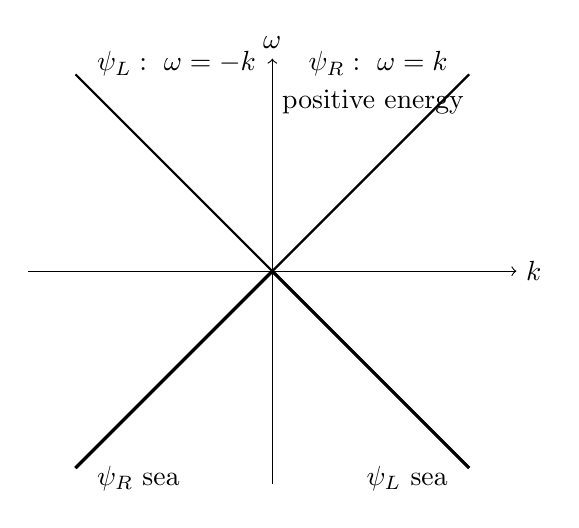
\begin{tikzpicture}[scale=1.0]
\draw[->] (-3.1,0) -- (3.1,0) node[right] {$k$};
\draw[->] (0,-2.7) -- (0,2.7) node[above] {$\omega$};
\draw[thick] (-2.5,-2.5) -- (2.5,2.5);
\draw[thick] (-2.5,2.5) -- (2.5,-2.5);
\draw[very thick] (-2.5,-2.5) -- (0,0);
\draw[very thick] (0,0) -- (2.5,-2.5);
\node[above left] at (2.35,2.35) {$\psi_R:\ \omega=k$};
\node[above right] at (-2.35,2.35) {$\psi_L:\ \omega=-k$};
\node[right] at (0,2.15) {positive energy};
\node[below right] at (-2.35,-2.35) {$\psi_R$ sea};
\node[below left] at (2.35,-2.35) {$\psi_L$ sea};
\end{tikzpicture}
\caption{Independent right- and left-moving fields give mirrored massless branches; the two negative-energy half-branches are filled in the vacuum.}
\end{figure}

After filling both negative-energy seas, there are as many left-moving as right-moving occupied states. Their vacuum momenta balance. Particle and hole excitations can now move in either direction.

\begin{classroomqa}
\lecturetimestamp{00:15:58}
\audiencequestion{Can the negative-energy problem be handled without postulating filled states and holes?}
\lecturerresponse{The same theory can be relabeled. A filled negative-energy electron state may be called an empty antiparticle state; then the physical language contains only positive-energy particles and antiparticles. The filled-sea picture remains a useful consistency check, much like a filled band in a metal, where removing an electron produces a hole while promotion produces both a particle and a hole.}
\end{classroomqa}

The excitations considered so far are massless. Their dispersions are linear and their velocities have magnitude \(1\), so they move at the speed of light. The next question is how to give them mass.

\section{Two Components and the Mass Term}

First combine the two fields into a column:
\begin{equation}
\Psi=
\begin{pmatrix}
\psi_R\\
\psi_L
\end{pmatrix}.
\end{equation}
This is initially only compact notation for two independent equations. Define
\begin{equation}
\alpha=
\begin{pmatrix}
1&0\\
0&-1
\end{pmatrix}.
\end{equation}
Then the right- and left-moving equations become
\begin{equation}
\frac{\partial\Psi}{\partial t}
=
-\alpha\frac{\partial\Psi}{\partial x}.
\end{equation}

\begin{figure}[htbp]
\centering

\includegraphics[width=0.78\textwidth]{lecture_06_figure_02.png}
\caption{The fields \(\psi_R\) and \(\psi_L\) form a two-component spinor, with \(\alpha\) distinguishing the two massless branches.}
\lectureframe{00:20:36}
\end{figure}

For a plane wave, the operators
\begin{equation}
i\partial_t
\quad\hbox{and}\quad
-i\partial_x
\end{equation}
return \(\omega\) and \(k\), respectively. The matrix equation may therefore be abbreviated as
\begin{equation}
\omega=\alpha k.
\end{equation}
For the upper component this says \(\omega=k\); for the lower component it says \(\omega=-k\). The notation has compressed the two equations but has introduced no new physics.

Electrons are not massless and do not move at the speed of light. A tempting formula for their energy is the nonrelativistic kinetic energy \(k^2/(2m)\), but that cannot be the starting point here: the massless limit already concerns motion at the speed of light. The relativistic relation is
\begin{equation}
\omega^2=k^2+m^2,
\end{equation}
or, including both energy branches,
\begin{equation}
\omega=\pm\sqrt{k^2+m^2}.
\end{equation}
When \(m=0\), these reduce to \(\omega=k\) and \(\omega=-k\).

\begin{classroomqa}
\lecturetimestamp{00:25:23}
\audiencequestion{Are units with \(c=1\) being used, and how is the speed of a massive particle obtained?}
\lecturerresponse{Yes. The speed of a wave packet is the group velocity, \(v_{\mathrm g}=d\omega/dk=k/\sqrt{k^2+m^2}\) on the positive-energy branch. Thus the dispersion relation itself contains the reduction of the speed below \(c=1\) for a massive particle.}
\end{classroomqa}

\begin{classroomqa}
\lecturetimestamp{00:26:29}
\audiencequestion{Is \(\omega\) a vector or a matrix in the shorthand \(\omega=\alpha k\)?}
\lecturerresponse{The shorthand stands for an operator equation acting on the two-component wavefunction. Here \(\omega\) means \(i\partial_t\), \(k\) means \(-i\partial_x\), and \(\alpha\) is the matrix acting on the component index. The scalar symbols \(\omega\) and \(k\) become their numerical eigenvalues only on a plane wave.}
\end{classroomqa}

Keep the equation first order and try the simplest mass-dependent extension:
\begin{equation}
\omega=\alpha k+\beta m.
\end{equation}
The object \(\beta\) must be a matrix because it acts on the same two-component field as \(\alpha\). Its algebra follows by squaring:
\begin{align}
\omega^2
&=(\alpha k+\beta m)(\alpha k+\beta m)\\
&=\alpha^2k^2+\beta^2m^2
+\alpha\beta\,km+\beta\alpha\,mk\\
&=\alpha^2k^2+\beta^2m^2
+(\alpha\beta+\beta\alpha)km.
\end{align}
To obtain \(k^2+m^2\) for every \(k\) and \(m\), require
\begin{equation}
\alpha^2=I,
\qquad
\beta^2=I,
\qquad
\alpha\beta+\beta\alpha=0.
\end{equation}

Two ordinary nonzero numbers cannot satisfy the last condition: for numbers it would give \(2\alpha\beta=0\), contrary to both squares being \(1\). Matrices can anticommute. In particular, \(\beta\) cannot equal \(\alpha\), since then
\begin{equation}
\alpha\beta+\beta\alpha=2\alpha^2=2I.
\end{equation}

Choose
\begin{equation}
\beta=
\begin{pmatrix}
0&1\\
1&0
\end{pmatrix}.
\end{equation}
Its square can be checked entry by entry:
\begin{equation}
\beta^2
=
\begin{pmatrix}
0&1\\
1&0
\end{pmatrix}
\begin{pmatrix}
0&1\\
1&0
\end{pmatrix}
=
\begin{pmatrix}
0\cdot0+1\cdot1&0\cdot1+1\cdot0\\
1\cdot0+0\cdot1&1\cdot1+0\cdot0
\end{pmatrix}
=
\begin{pmatrix}
1&0\\
0&1
\end{pmatrix}.
\end{equation}
The order of multiplication matters:
\begin{align}
\alpha\beta
&=
\begin{pmatrix}
1&0\\
0&-1
\end{pmatrix}
\begin{pmatrix}
0&1\\
1&0
\end{pmatrix}
=
\begin{pmatrix}
0&1\\
-1&0
\end{pmatrix},\\
\beta\alpha
&=
\begin{pmatrix}
0&1\\
1&0
\end{pmatrix}
\begin{pmatrix}
1&0\\
0&-1
\end{pmatrix}
=
\begin{pmatrix}
0&-1\\
1&0
\end{pmatrix}.
\end{align}
Thus
\begin{equation}
\alpha\beta=-\beta\alpha,
\qquad
\alpha\beta+\beta\alpha=0.
\end{equation}
Other equivalent matrix choices are possible, but this one makes the component equations especially transparent.

Restoring the differential operators gives the massive equation
\begin{equation}
i\frac{\partial\Psi}{\partial t}
=
-i\alpha\frac{\partial\Psi}{\partial x}
+m\beta\Psi.
\end{equation}
The matrix \(\beta\) interchanges the two components:
\begin{equation}
\beta
\begin{pmatrix}
\psi_R\\
\psi_L
\end{pmatrix}
=
\begin{pmatrix}
\psi_L\\
\psi_R
\end{pmatrix}.
\end{equation}
Consequently,
\begin{align}
i\dot{\psi}_R
&=-i\frac{\partial\psi_R}{\partial x}+m\psi_L,\\
i\dot{\psi}_L
&=+i\frac{\partial\psi_L}{\partial x}+m\psi_R.
\end{align}

The mass term couples fields that were independent in the massless theory. The equation for the upper component contains the lower component, and the equation for the lower component contains the upper one. This coupling is what a Dirac mass means. The equations are translation invariant, so they conserve momentum, and the mass of their particle excitations is \(m\).

\begin{classroomqa}
\lecturetimestamp{00:38:25}
\audiencequestion{Is a solution automatically Lorentz invariant?}
\lecturerresponse{A particular solution should not remain fixed under a Lorentz transformation. A state with one momentum is carried into a state with the transformed momentum, so the appropriate statement is covariance. The relation \(\omega^2=k^2+m^2\) is one key Lorentz-invariant check, but full covariance also requires the transformation law of the spinor \(\Psi\), which has not yet been established.}
\end{classroomqa}

\section{The Rest Frame and the Meaning of the Components}

A massless particle cannot be brought to rest, but a massive particle can. At rest \(k=0\), so the wavefunction has no spatial variation and
\begin{equation}
\omega=\beta m.
\end{equation}
The differential equation reduces to
\begin{equation}
i\frac{d\Psi}{dt}=m\beta\Psi.
\end{equation}
In components,
\begin{align}
i\dot{\psi}_R&=m\psi_L,\\
i\dot{\psi}_L&=m\psi_R.
\end{align}
Both off-diagonal entries of \(\beta\) are \(+1\), so there is no extra minus sign in either of these equations.

The equations decouple after adding and subtracting the components. Define
\begin{equation}
\psi_+=\psi_R+\psi_L,
\qquad
\psi_-=\psi_R-\psi_L.
\end{equation}
Adding the two rest-frame equations gives
\begin{equation}
i\dot{\psi}_+=m\psi_+,
\end{equation}
while subtracting them gives
\begin{equation}
i\dot{\psi}_-=-m\psi_-.
\end{equation}
Thus
\begin{equation}
\omega=+m
\quad\hbox{for }\psi_+,
\qquad
\omega=-m
\quad\hbox{for }\psi_-.
\end{equation}

\begin{figure}[htbp]
\centering

\includegraphics[width=0.62\textwidth]{lecture_06_figure_03.png}
\caption{At zero momentum, \(\psi_+=\psi_R+\psi_L\) and \(\psi_-=\psi_R-\psi_L\) have rest frequencies \(\omega=+m\) and \(\omega=-m\).}
\lectureframe{00:44:49}
\end{figure}

The positive-energy rest field is \(\psi_+\); the negative-energy rest field is \(\psi_-\). The negative-energy states are filled, just as before. The rest-frame result is only the \(k=0\) slice of the full spectrum:
\begin{equation}
\omega_\pm(k)=\pm\sqrt{k^2+m^2}.
\end{equation}
\begin{figure}[htbp]
\centering
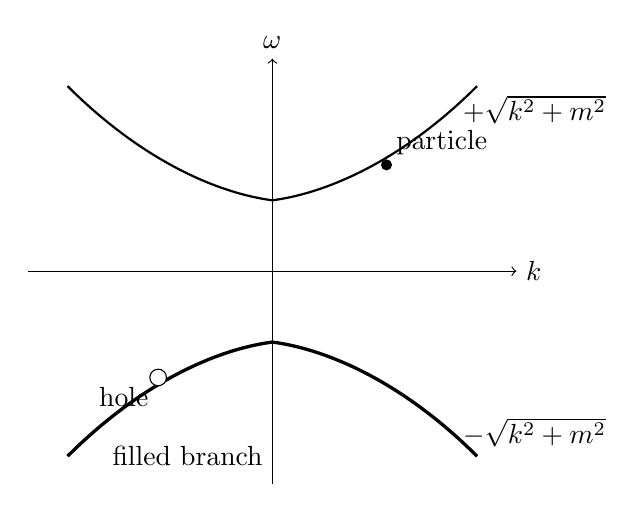
\begin{tikzpicture}[scale=1.0]
\draw[->] (-3.1,0) -- (3.1,0) node[right] {$k$};
\draw[->] (0,-2.7) -- (0,2.7) node[above] {$\omega$};
\draw[thick] (-2.6,2.35)
  .. controls (-1.7,1.45) and (-0.75,1.0) .. (0,0.9)
  .. controls (0.75,1.0) and (1.7,1.45) .. (2.6,2.35);
\draw[very thick] (-2.6,-2.35)
  .. controls (-1.7,-1.45) and (-0.75,-1.0) .. (0,-0.9)
  .. controls (0.75,-1.0) and (1.7,-1.45) .. (2.6,-2.35);
\fill (1.45,1.35) circle (2pt);
\node[above right] at (1.45,1.35) {particle};
\fill[white] (-1.45,-1.35) circle (3pt);
\draw (-1.45,-1.35) circle (3pt);
\node[below left] at (-1.45,-1.35) {hole};
\node[right] at (2.3,2.05) {$+\sqrt{k^2+m^2}$};
\node[right] at (2.3,-2.05) {$-\sqrt{k^2+m^2}$};
\node[left] at (0,-2.35) {filled branch};
\end{tikzpicture}
\caption{At every momentum the massive spectrum has positive- and negative-energy states. The negative branch is filled, and a missing state in it is a positive-energy hole.}
\end{figure}
Every momentum has a positive- and a negative-energy state. Filling every state on the negative branch leaves positive-energy particles above the sea and positive-energy holes in it. Particles and holes both have positive mass.

The essential point deserves repetition. A fermion becomes massive when its two formerly independent components are coupled. At rest, neither original component alone is an energy eigenstate. The definite-energy states are their sum and difference.

To see what the sum means, write \(C_R^\dagger\) and \(C_L^\dagger\) for the relevant one-particle creation pieces. Acting on the vacuum,
\begin{equation}
(C_R^\dagger+C_L^\dagger)\lvert0\rangle
\end{equation}
creates one particle in a coherent superposition of the two components. It does not create two particles. A product,
\begin{equation}
C_R^\dagger C_L^\dagger\lvert0\rangle,
\end{equation}
contains two creation operators and creates a two-particle state when both modes are available. After normalization, the rest state has equal probability in the two components, but the coupled wave as a whole has zero momentum.

The labels \(R\) and \(L\) were literal motion labels only when \(m=0\). Once the mass term is present, a moving massive solution generally contains both components, and the rest solution contains them with equal magnitude. It is therefore better to regard \(R\) and \(L\) here as labels for the upper and lower spinor components.

\begin{figure}[htbp]
\centering

\includegraphics[width=0.78\textwidth]{lecture_06_figure_04.png}
\caption{For nonzero mass, the two spinor components are coupled; their right- and left-moving interpretation applies directly only in the massless limit.}
\lectureframe{00:50:48}
\end{figure}

All massive fermions in particle physics are built from left- and right-component fields: a Dirac mass couples components that are independent in the massless limit.

\begin{classroomqa}
\lecturetimestamp{00:52:01}
\audiencequestion{Should \(\psi_R\pm\psi_L\) include a factor of \(1/\sqrt{2}\)?}
\lecturerresponse{It may be included to normalize the state. It multiplies both sides of the equation and therefore does not change the equation of motion.}
\end{classroomqa}

\begin{classroomqa}
\lecturetimestamp{00:52:12}
\audiencequestion{Do the relative magnitudes of the right and left components matter?}
\lecturerresponse{For the chosen rest-frame eigenstates their magnitudes are equal. An overall normalization is arbitrary, but the relative magnitudes are fixed by the eigenvector of \(\beta\).}
\end{classroomqa}

\begin{classroomqa}
\lecturetimestamp{00:52:52}
\audiencequestion{Could the two components have a relative phase?}
\lecturerresponse{Yes. The real coefficients in \(\psi_R\pm\psi_L\) follow from choosing a real \(\beta\). Other matrices that square to the identity and anticommute with \(\alpha\) are equivalent choices, and phases may then appear between the components. Once a representation is chosen, it must be used consistently.}
\end{classroomqa}

\begin{classroomqa}
\lecturetimestamp{00:53:43}
\audiencequestion{Are ``left mover'' and ``right mover'' misleading labels after mass is added?}
\lecturerresponse{Somewhat. They describe genuine left- and right-moving waves in the massless theory. With nonzero mass, even a particle moving in one direction generally contains both components, so ``upper component'' and ``lower component'' are safer labels.}
\end{classroomqa}

\begin{classroomqa}
\lecturetimestamp{00:55:01}
\audiencequestion{Does a fermion at rest already require spin angular momentum?}
\lecturerresponse{Not in this one-dimensional model. Angular momentum is not defined in one spatial dimension, so spin has not yet entered the construction.}
\end{classroomqa}

\begin{classroomqa}
\lecturetimestamp{00:55:24}
\audiencequestion{Does the wavefunction contain fermionic creation and annihilation operators?}
\lecturerresponse{Yes.}
\end{classroomqa}

\begin{classroomqa}
\lecturetimestamp{00:55:30}
\audiencequestion{Where does the fermionic character enter apart from the choice of creation and annihilation operators?}
\lecturerresponse{It enters through the fermionic creation--annihilation rules. An equation with this negative-energy spectrum has to be quantized with those rules; bosonic occupation rules would leave the vacuum unstable. Relativistic bosons must be described by a different wave equation.}
\end{classroomqa}

\begin{classroomqa}
\lecturetimestamp{00:56:20}
\audiencequestion{Can a nonzero-momentum solution be Lorentz-transformed into the rest-frame solution?}
\lecturerresponse{Yes. A boost can carry a massive solution to its rest frame, but carrying out the transformation requires knowing how Lorentz transformations act on the spinor \(\Psi\).}
\end{classroomqa}

\section{Mass from a Scalar Vacuum Field}

\begin{classroomqa}
\lecturetimestamp{00:58:11}
\audiencequestion{How does interaction with the Higgs field produce the Dirac mass term?}
\lecturerresponse{Replace the constant mass coefficient by a coupling to a scalar field. If that field vanishes in the vacuum, the fermion remains massless; if it has a constant nonzero vacuum value, the coupling acts exactly like a mass.}
\end{classroomqa}

Let \(\phi(x,t)\) be a scalar field with its own equation of motion. In the Dirac equation, replace the constant \(m\) in the mass term by \(g\phi(x,t)\):\footnote{The displayed interaction term is obtained by making this substitution in the previously established mass term \(m\beta\Psi\).}
\begin{equation}
i\frac{\partial\Psi}{\partial t}
=
-i\alpha\frac{\partial\Psi}{\partial x}
+g\phi(x,t)\,\beta\Psi.
\end{equation}
The two field equations are then coupled. The fermion acts on the scalar field, and the scalar field acts back on the fermion; considered together, the system is nonlinear even though the Dirac equation is linear in \(\Psi\) for a prescribed \(\phi\).

Suppose first that empty space has
\begin{equation}
\phi(x,t)=0.
\end{equation}
Then the mixing term vanishes, the upper and lower components decouple, and the fermion is massless. Suppose instead that the lowest-energy state has a constant nonzero scalar field,
\begin{equation}
\phi(x,t)=\phi_0\neq0.
\end{equation}
The Dirac equation in that vacuum becomes
\begin{equation}
i\frac{\partial\Psi}{\partial t}
=
-i\alpha\frac{\partial\Psi}{\partial x}
+g\phi_0\,\beta\Psi,
\end{equation}
so that
\begin{equation}
m_{\mathrm{eff}}=g\phi_0.
\end{equation}
A coupling between a bosonic field and a fermionic field, together with a nonzero value of the bosonic field in empty space, therefore generates the same left-right mixing that previously appeared as a mass written directly into the equation.

\begin{classroomqa}
\lecturetimestamp{01:01:27}
\audiencequestion{Could the LHC provide evidence for a nonzero Higgs field in the vacuum?}
\lecturerresponse{Absolutely. That is one of the big issues.}
\end{classroomqa}

\begin{classroomqa}
\lecturetimestamp{01:01:32}
\audiencequestion{Can you say more about how the Higgs mechanism works?}
\lecturerresponse{A scalar field has energy associated with its space and time variation, and it may also have a local potential energy \(V(\phi)\). If the minima of that potential occur at nonzero values of \(\phi\), the vacuum contains a nonzero field. Quantized oscillations about the chosen minimum are Higgs particles.}
\end{classroomqa}

A field can carry energy in two distinct ways. Some energy depends on how the field varies in space and time. The Maxwell field is the familiar comparison:
\begin{equation}
\mathcal{E}_{\mathrm{Maxwell}}\propto \mathbf E^2+\mathbf B^2,
\end{equation}
and both \(\mathbf E\) and \(\mathbf B\) are built from derivatives of the electromagnetic potential. Thus this energy is associated with space and time variation of the underlying field.

A scalar field can also have a local potential-energy density,
\begin{equation}
V(\phi),
\end{equation}
which depends on the value of \(\phi\) itself rather than on its derivatives. Schematically,
\begin{equation}
\mathcal{E}_\phi
=
\mathcal E_{\text{space and time gradients}}+V(\phi).
\end{equation}
Without a deeper principle fixing it, \(V(\phi)\) could be any reasonable function compatible with the symmetries of the model.

For the simplified real-scalar illustration being used here, take the theory to be symmetric under
\begin{equation}
\phi\longrightarrow-\phi.
\end{equation}
The potential must then be even:
\begin{equation}
V(\phi)=V(-\phi).
\end{equation}
This symmetry alone does not say where the minimum lies. One possibility is a single minimum at \(\phi=0\). Another is a symmetric pair of minima at nonzero values, one positive and one negative.

\begin{figure}[htbp]
\centering

\includegraphics[width=0.72\textwidth]{lecture_06_figure_05.png}
\caption{A minimum at \(\phi=0\) gives a vanishing vacuum field, whereas symmetric nonzero minima permit a vacuum value \(\phi_0\neq0\) and hence a fermion mass \(g\phi_0\).}
\lectureframe{01:04:47}
\end{figure}

The two possibilities can be drawn without committing to a particular polynomial form for the potential.\footnote{The curves below retain only the qualitative centered and symmetry-related minima used in the argument.}
\begin{figure}[htbp]
\centering
\begin{tikzpicture}[x=1.35cm,y=1.05cm]
\begin{scope}[shift={(-3.1,0)}]
\draw[->] (-1.7,0) -- (1.7,0) node[right] {$\phi$};
\draw[->] (0,-0.15) -- (0,2.45) node[above] {$V(\phi)$};
\draw[thick] (-1.5,2.05) .. controls (-0.9,0.65) and (-0.45,0.25) .. (0,0.25)
             .. controls (0.45,0.25) and (0.9,0.65) .. (1.5,2.05);
\fill (0,0.25) circle (1.2pt);
\node[below] at (0,0) {$0$};
\end{scope}
\begin{scope}[shift={(3.1,0)}]
\draw[->] (-1.7,0) -- (1.7,0) node[right] {$\phi$};
\draw[->] (0,-0.15) -- (0,2.45) node[above] {$V(\phi)$};
\draw[thick] (-1.55,2.05)
  .. controls (-1.25,0.75) and (-1.0,0.25) .. (-0.75,0.25)
  .. controls (-0.35,0.25) and (-0.25,1.3) .. (0,1.3)
  .. controls (0.25,1.3) and (0.35,0.25) .. (0.75,0.25)
  .. controls (1.0,0.25) and (1.25,0.75) .. (1.55,2.05);
\fill (-0.75,0.25) circle (1.2pt);
\fill (0.75,0.25) circle (1.2pt);
\node[below] at (0,0) {$0$};
\node[below] at (-0.75,0) {$-\phi_0$};
\node[below] at (0.75,0) {$\phi_0$};
\end{scope}
\end{tikzpicture}
\caption{Even potentials may have a centered minimum or two symmetry-related nonzero minima.}
\end{figure}

If the minimum is at the origin, the vacuum has \(\phi_0=0\), and this coupling gives the electron no mass. If the minima are at \(\phi=\pm\phi_0\), the vacuum settles into either one. The two choices are related by the symmetry, and either produces a nonzero coefficient \(g\phi_0\) in the Dirac equation. Why the potential has this qualitative shape is a deeper question, not settled by the mechanism itself.

The field need not remain exactly at its minimum. It can oscillate about the chosen value just as a particle can oscillate near the bottom of a potential well. Quantizing those oscillations gives Higgs quanta. Their characteristic frequency is related to the Higgs-particle mass: a large mass means that a large amount of energy is needed to excite even one quantum. In the vacuum the field simply sits near its minimum and supplies the fermion mass. When the field vibrates, the vibration is a Higgs particle.

The coupling entails action and reaction. Fermions respond to the value of \(\phi\), but sufficiently energetic fermion collisions can also excite the scalar field. A collision must supply the excitation energy; once the field is vibrating, its quanta are Higgs particles. The same field couples not only to electrons but also to quark fields and other fields whose masses it supplies.

\begin{classroomqa}
\lecturetimestamp{01:08:14}
\audiencequestion{If the Higgs field vibrates or is displaced, does the electron mass change?}
\lecturerresponse{Yes. Since the effective mass is proportional to the local value of the field, displacing the field toward zero reduces the mass. Holding a macroscopic region far from the vacuum value would require enormous energy; a region large enough for such an experiment could collapse into a black hole.}
\end{classroomqa}

The thought experiment is direct. If a region could be held near \(\phi=0\), then within that region
\begin{equation}
m_{\mathrm{eff}}=g\phi
\end{equation}
would become small or vanish. An excited Higgs mode oscillates about the vacuum value, whereas producing and maintaining an appreciable displacement throughout a macroscopic region requires enormous energy. The potential-energy cost grows with the volume. Long before such a region became a practical laboratory, its energy could be large enough for gravitational collapse. The change of mass is real in principle, but arranging a large observable change is fantastically difficult.

\begin{classroomqa}
\lecturetimestamp{01:09:27}
\audiencequestion{Why is a Higgs field needed?}
\lecturerresponse{Because the electron has mass.}
\end{classroomqa}

\begin{classroomqa}
\lecturetimestamp{01:09:41}
\audiencequestion{Does each kind of particle have its own Higgs field?}
\lecturerresponse{No. In the Standard Model one Higgs field supplies masses to electrons, quarks, and the other particles participating in this mechanism. Supersymmetric versions require two Higgs fields rather than one separate field for every particle species.}
\end{classroomqa}

The one-field picture is schematic: the full Higgs field has more structure than a single real number \(\phi\). Nevertheless the essential point survives. A common vacuum field can couple with different strengths to different fermions, so different masses do not require different Higgs fields for every species. The Higgs particle is an oscillation of that same field about its vacuum value.

Why not simply put the electron mass into the equation by hand and dispense with the Higgs field? The answer has to do with the weak interactions and unification, and it is deferred.

\begin{classroomqa}
\lecturetimestamp{01:11:16}
\audiencequestion{In a supersymmetric theory, are there two Higgs sectors?}
\lecturerresponse{Yes. In the simplified division used here, one supplies masses to up-type quarks and the other to down-type quarks and electrons. The doubling is a technical requirement of supersymmetry, not a separate Higgs field for every particle.}
\end{classroomqa}

\begin{classroomqa}
\lecturetimestamp{01:12:01}
\audiencequestion{If the Higgs particle has mass, where does that mass come from?}
\lecturerresponse{That question is not resolved here. The sharper puzzle is why the Higgs mass is so small.}
\end{classroomqa}

Symmetry is inseparable from the problem of mass. In the simple Dirac model, a symmetry that keeps the left and right sectors from mixing would force the coefficient of the mixing term to vanish. If the vacuum respected that symmetry, the fermion would be massless. A nonzero Higgs vacuum value breaks the relevant vacuum symmetry and permits the left-right coupling:
\begin{equation}
m_{\mathrm{eff}}=g\phi_0\neq0.
\end{equation}
The precise symmetry transformation is not developed here; the point is its consequence for the mass term. The equations may possess the symmetry even though the particular lowest-energy state does not. It is this asymmetry of the vacuum that supplies the mass.

In the electroweak picture being sketched, electrons and quarks acquire mass in this way, as do the \(W\) and \(Z\) bosons. The photon remains massless. The Higgs particle itself is another exception: it can have mass even without the same vacuum displacement, and its mass concerns oscillations of its own field rather than left-right fermion mixing. Thus the Higgs vacuum value generates the masses of the other particles in this account, while the mass of the Higgs excitation raises a separate question.

\begin{classroomqa}
\lecturetimestamp{01:15:26}
\audiencequestion{Does the graviton have mass?}
\lecturerresponse{No. The graviton is massless, like the photon. Neutrinos were once also thought to be massless, but they have a very small mass; in the present language that means that their left and right components have only a very small coupling.}
\end{classroomqa}

Photons and, in the theory, gravitons are massless and move at the speed of light. Neutrinos do not quite belong to that class. Their tiny mass means, in this Dirac language, that the coupling which joins their left and right components is tiny. Why it is so small is another question.

\section{The Dirac Equation in Three Spatial Dimensions}

In three spatial dimensions the wave number becomes a wave vector,
\begin{equation}
\mathbf{k}=(k_1,k_2,k_3),
\end{equation}
with components along the \(x\), \(y\), and \(z\) directions. The one-dimensional relation has the sign
\begin{equation}
\omega=\alpha k+\beta m,
\end{equation}
and its simplest linear generalization is
\begin{equation}
\omega
=
\alpha_1 k_1+\alpha_2 k_2+\alpha_3 k_3+\beta m.
\end{equation}
Here the \(\alpha_i\) and \(\beta\) are matrices. They must be chosen so that
\begin{equation}
\omega^2=k_1^2+k_2^2+k_3^2+m^2.
\end{equation}
This invariant dispersion relation is an essential condition, although by itself it is not the whole content of relativity.

Squaring the linear expression gives
\begin{align}
\omega^2
={}&
\alpha_1^2k_1^2+\alpha_2^2k_2^2+\alpha_3^2k_3^2+\beta^2m^2
\nonumber\\
&+(\alpha_1\alpha_2+\alpha_2\alpha_1)k_1k_2
+(\alpha_1\alpha_3+\alpha_3\alpha_1)k_1k_3
\nonumber\\
&+(\alpha_2\alpha_3+\alpha_3\alpha_2)k_2k_3
+\sum_{i=1}^{3}(\alpha_i\beta+\beta\alpha_i)k_i m.
\end{align}
The coefficients of the squared momenta and the mass require
\begin{equation}
\alpha_1^2=\alpha_2^2=\alpha_3^2=I,
\qquad
\beta^2=I.
\end{equation}
The unwanted \(k_i k_j\) terms disappear if distinct \(\alpha\) matrices anticommute:
\begin{equation}
\alpha_i\alpha_j+\alpha_j\alpha_i=0,
\qquad i\neq j.
\end{equation}
The mixed \(k_i m\) terms disappear if
\begin{equation}
\alpha_i\beta+\beta\alpha_i=0
\qquad
\text{for each }i.
\end{equation}
Thus all four matrices square to the identity, and every pair of distinct matrices anticommutes.

Three \(2\times2\) matrices with the required mutual anticommutation properties do exist: they are the three Pauli matrices. There is no fourth \(2\times2\) matrix that both squares to the identity and anticommutes with all three. No \(3\times3\) realization works either. The first possible realization uses \(4\times4\) matrices, the Dirac matrices.

The passage from two components to four raises a physical question. In one spatial dimension the two components began as right- and left-moving fields. What do four components mean? The new ingredient will be spin, but spin requires angular momentum and therefore a genuine three-dimensional discussion.

The matrices are not unique. Different choices are equivalent in much the same way that different choices of mutually orthogonal coordinate axes are equivalent: the entries change, but a transformation relates the descriptions and the physics is unchanged. One convenient representation is\footnote{The entrywise matrices below are the expansion of the block form and Pauli matrices displayed immediately afterward; those block relations are stated explicitly in the lecture at 01:30:23--01:31:29.}
\begin{equation}
\beta=
\begin{pmatrix}
1&0&0&0\\
0&1&0&0\\
0&0&-1&0\\
0&0&0&-1
\end{pmatrix},
\end{equation}
together with
\begin{align}
\alpha_1&=
\begin{pmatrix}
0&0&0&1\\
0&0&1&0\\
0&1&0&0\\
1&0&0&0
\end{pmatrix},
&
\alpha_2&=
\begin{pmatrix}
0&0&0&-i\\
0&0&i&0\\
0&-i&0&0\\
i&0&0&0
\end{pmatrix},
\\[1ex]
\alpha_3&=
\begin{pmatrix}
0&0&1&0\\
0&0&0&-1\\
1&0&0&0\\
0&-1&0&0
\end{pmatrix}.
\end{align}
Their structure is easier to see by dividing each matrix into \(2\times2\) blocks:
\begin{equation}
\beta=
\begin{pmatrix}
I_2&0\\
0&-I_2
\end{pmatrix},
\qquad
\alpha_i=
\begin{pmatrix}
0&\sigma_i\\
\sigma_i&0
\end{pmatrix}.
\end{equation}
The three Pauli matrices are
\begin{equation}
\sigma_1=
\begin{pmatrix}
0&1\\
1&0
\end{pmatrix},
\qquad
\sigma_2=
\begin{pmatrix}
0&-i\\
i&0
\end{pmatrix},
\qquad
\sigma_3=
\begin{pmatrix}
1&0\\
0&-1
\end{pmatrix}.
\end{equation}
These block matrices obey the required Dirac anticommutation relations.

The wavefunction must now have four components:
\begin{equation}
\Psi=
\begin{pmatrix}
\psi_1\\
\psi_2\\
\psi_3\\
\psi_4
\end{pmatrix}.
\end{equation}
The equation of motion is
\begin{equation}
i\frac{\partial\Psi}{\partial t}
=
-i\sum_{j=1}^{3}\alpha_j
\frac{\partial\Psi}{\partial x_j}
+\beta m\Psi.
\end{equation}
This compact expression stands for four coupled linear differential equations. The off-diagonal entries of the \(\alpha_j\) mix the four components in a more intricate way than in the one-dimensional case, but the basic structure is the same: matrices couple the components while the equation remains first order in space and time. The additional doubling of components is the clue that leads to spin.

\begin{classroomqa}
\lecturetimestamp{01:33:53}
\audiencequestion{Are the four components of \(\Psi\) a four-vector associated directly with the four dimensions of spacetime?}
\lecturerresponse{No. They form a spinor, not a four-vector. The equality between the two spacetime dimensions and the two spinor components in the one-dimensional example was accidental. In higher-dimensional constructions the spinor matrix sizes occur in powers of two and do not in general equal the number of spacetime dimensions.}
\end{classroomqa}

The rest frame again gives the simplest interpretation. At zero momentum the derivative term vanishes:
\begin{equation}
i\frac{\partial\Psi}{\partial t}=m\beta\Psi.
\end{equation}
In the chosen representation, \(\beta\) has two eigenvalues \(+1\) and two eigenvalues \(-1\). There are therefore two rest states with energy \(+m\) and two with energy \(-m\). As before, the negative-energy states are filled. The twofold multiplicity within each energy sign is the extra structure whose physical interpretation is spin.

\begin{classroomqa}
\lecturetimestamp{01:35:51}
\audiencequestion{Should the off-diagonal blocks in \(\alpha_i\) carry the same index, so that they are \(\sigma_i\)?}
\lecturerresponse{Yes. Each matrix \(\alpha_i\) contains the corresponding Pauli matrix \(\sigma_i\) in both off-diagonal blocks.}
\end{classroomqa}

\begin{classroomqa}
\lecturetimestamp{01:36:03}
\audiencequestion{Is a factor of two missing in the compact anticommutation relation for the \(\alpha_i\)?}
\lecturerresponse{Yes. When \(i=j\), the left-hand side is \(\alpha_i^2+\alpha_i^2=2I\). The correct relation is \(\alpha_i\alpha_j+\alpha_j\alpha_i=2\delta_{ij}I\).}
\end{classroomqa}

The separate square and unequal-index conditions can therefore be combined as
\begin{equation}
\alpha_i\alpha_j+\alpha_j\alpha_i=2\delta_{ij}I.
\end{equation}

\begin{classroomqa}
\lecturetimestamp{01:36:42}
\audiencequestion{Was the move to four matrices a major conceptual leap in Dirac's construction?}
\lecturerresponse{Yes. Dirac postulated the equation and followed its consequences. One consequence was the appearance of antiparticles; another was spin. Spin was already known empirically, but the equation accounted for it.}
\end{classroomqa}

\begin{classroomqa}
\lecturetimestamp{01:37:29}
\audiencequestion{Did the empirical evidence or the theorem restricting particles to bosons and fermions come first?}
\lecturerresponse{The empirical evidence came first and the theorem later. The boson--fermion alternative applies in three spatial dimensions. In two spatial dimensions, with one time dimension, intermediate statistics can occur; in \(3+1\) dimensions, and in higher spatial dimensions, the alternatives are bosons and fermions.}
\end{classroomqa}

\begin{classroomqa}
\lecturetimestamp{01:39:01}
\audiencequestion{Is there a customary index for the four components of \(\Psi\)?}
\lecturerresponse{No essential choice is fixed here. The labels \(p\) and \(q\) may be used, running from one to four; each matrix then has one row index and one column index.}
\end{classroomqa}

Matrix notation suppresses these component labels. If they are exposed, then
\begin{equation}
p,q=1,2,3,4,
\end{equation}
and the equation reads
\begin{equation}
i\,\partial_t\Psi_p
=
-i\sum_{j=1}^{3}\sum_{q=1}^{4}
(\alpha_j)_{pq}\,\partial_j\Psi_q
+m\sum_{q=1}^{4}\beta_{pq}\Psi_q.
\end{equation}

\begin{classroomqa}
\lecturetimestamp{01:40:15}
\audiencequestion{Are the explicit component indices unnecessary when matrix multiplication is used?}
\lecturerresponse{Yes. Matrix notation suppresses those indices automatically. A more symmetric form that makes the relativistic structure more explicit can be introduced later.}
\end{classroomqa}

The displayed equation is the Dirac equation in its simplest \(3+1\)-dimensional form. The next steps are to understand spin and to construct the wave equations for relativistic bosons, since the Dirac equation is not their equation and about half the particles in nature are bosons. With those ingredients in place, one can turn to quarks, leptons, weak bosons, Higgs particles, and photons, and bring some order to the particle spectrum. More symmetry is needed throughout that discussion.
